\documentclass[10 pt]{article}
\usepackage{tikz}
\usetikzlibrary{arrows}
\usepackage[margin=0.5 in]{geometry}
\usepackage[utf8]{inputenc}
\usepackage{tabu}
\usepackage{color}
\usepackage{xcolor}
\usepackage{listings}
\usepackage{enumitem}
\usepackage{multicol}
\setlength{\columnsep}{1cm} 
\title{\textbf {Estructuras de Datos 1 - ST0245\\Segundo Parcial Grupo 032 (Martes)}}
\author{Nombre ..............................\\
		Departamento de Informática y Sistemas\\
		Universidad EAFIT\\}
\date{Mayo 8 de 2018}
\begin{document}
\lstdefinestyle{customc}{
	language=Java, 
	numbers=left, 
	showspaces=false,
    showstringspaces=false, 
    tabsize=2, 
    breaklines=true,
    xleftmargin=5.0ex,
}
\lstset{escapechar=@,style=customc, numbers=left, stepnumber = 1} 
\maketitle
\begin{multicols}{2}
Para propósitos de éste parcial se considerará la implementación de un árbol binario y sus respectivos recorridos.
\begin{lstlisting}
//Arbol binario
class BNode{
  BNode izq;
  BNode der;
  int val;
}

//Recorridos
void preorden(BNode nodo){
  if(nodo != null){
    System.out.println(nodo.val);
    preorden(nodo.izq);
    preorden(nodo.der);  
  }
}
void posorden(BNode nodo){
  if(nodo != null){
    posorden(nodo.izq);
    posorden(nodo.der);
    System.out.println(nodo.val);  
  }
}
void inorden(BNode nodo){
  if(nodo != null){
    inorden(nodo.izq);
    System.out.println(nodo.val);
    inorden(nodo.der);  
  }
}

\end{lstlisting}
\section{Pilas 30\%}
El método \texttt{push(i)} ingresa el elemento $i$ al tope de la pila. El método \texttt{pop()} retira
el elemento en el tope de la pila y retorna su valor. Considere el siguiente método:

\begin{lstlisting}
void metodo(int n, int x){
  Stack<Integer> s = new Stack();
  for(int i = 0; i < n; i++){
    if(i % 3 == 0){  
      s.push(i);    
    }  
  }
  int k = 0;
  while(s.size() > 0){
    if( k == x ){
      System.out.println(s.pop());
      break;    
    }
    k = k + 2;
    s.pop();
  }
}
\end{lstlisting}
\begin{enumerate}[label=\alph*]
\item (10\%) ¿Cuál es la complejidad asintótica, en el peor de los casos, del algoritmo anterior?
\begin{enumerate}[label=(\roman*)]
\item $O(\log n)$
\item $O(1)$
\item $O(n ^ 2)$
\item $O(n)$
\end{enumerate}
\item (10\%) ¿Qué valor imprime el algoritmo anterior cuando $x = 8$ y $ n = 20$?
\begin{enumerate}[label=(\roman*)]
\item 6
\item 8
\item 12
\item 3
\end{enumerate}
\item (10\%) ¿Cuál es la complejidad asintótica, en el peor de los casos, de encontrar un elemento en un pila con $n$ elementos, en otras palabras, decir si un elemento está o no está en la pila?
\begin{enumerate}[label=(\roman*)]
\item $O(1)$
\item $O(n)$
\item $O(\log n)$
\item $O(n^2)$
\end{enumerate}
\end{enumerate}
\section{Árboles 30\%}
\begin{center}
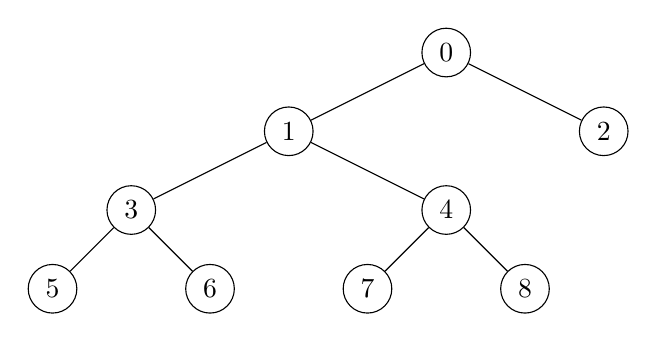
\begin{tikzpicture}

\tikzset{vertex/.style = {shape=circle,draw,minimum size=1.5em}}
\tikzset{edge/.style = {-,> = latex'}}
\node[vertex] (0) at (0,0)  {0};
\node[vertex] (1) at (-2,-1)  {1};
\node[vertex] (2) at (2, -1) {2};
\node[vertex] (3) at (-4, -2) {3};
\node[vertex] (4) at (0, -2) {4};
\node[vertex] (5) at (-5, -3) {5};
\node[vertex] (6) at (-3, -3) {6};
\node[vertex] (7) at (-1, -3) {7};
\node[vertex] (8) at (1, -3) {8};

%edges
\draw[edge] (0) to (1);
\draw[edge] (0) to (2);
\draw[edge] (1) to (3);
\draw[edge] (1) to (4);
\draw[edge] (3) to (5);
\draw[edge] (3) to (6);
\draw[edge] (4) to (7);
\draw[edge] (4) to (8);
\end{tikzpicture}
\end{center}

\begin{enumerate}[label=\alph*]
\item (10\%) Sean $A$ y $B$ las salidas de los recorridos pre-orden y pos-orden del árbol binario anterior, respectivamente. Determine el numero de elementos para los cuales se cumple que $A_i = B_i$ para $1 \leq i \leq 8$.
\begin{enumerate}[label=(\roman*)]
\item 3
\item 2
\item 4
\item 0
\end{enumerate}
\item (10\%) ¿Cuál es la salida del recorrido in-orden del árbol binario anterior?
\begin{enumerate}[label=(\roman*)]
\item 5, 3, 6, 1, 7, 4, 8, 0, 2
\item 0, 1, 3, 5, 6, 4, 7, 8, 2
\item 5, 6, 3, 7, 8, 4, 1, 2, 0
\item 5, 6, 3, 1, 7, 4, 8, 0, 2  
\end{enumerate}
\item (10\%) ¿Es un \textbf{\textit{árbol binario de búsqueda}} el árbol anterior?
\begin{enumerate}[label=(\roman*)]
\item Sí
\item No
\end{enumerate}
\end{enumerate}
\section{Colas 30\%}
El método \texttt{add(i)} agrega el elemento $i$ al inicio de la cola. El método \texttt{poll()} retira el elemento al final de la cola y retorna su valor. Considere el siguiente método:
\begin{lstlisting}
void calcular(int k){
  Queue<Integer> q = new Queue();
  for(int i = 0; i < k; ++i){
    if(k % 3 == 0 && i % 3 == 0){
      q.add(k - i);
    }  
  }
  int j = 0;
  while(q.size() > 0){
    if(j == 3){
      System.out.println(q.poll());
      break;    
    }  
    q.poll();
    j++;
  }
}
\end{lstlisting}
\begin{enumerate}[label=\alph*]
\item (10\%) ¿Cuál es la complejidad asintótica, en el peor de los casos, del algoritmo anterior?
\begin{enumerate}[label=(\roman*)]
\item $O(k)$
\item $O(k^2)$
\item $O(n \log k)$
\item $O(1)$
\end{enumerate}
\item (10\%) ¿Qué imprime el algoritmo anterior cuando $k = 21$?
\begin{enumerate}[label=(\roman*)]
\item 6
\item 9
\item 12
\item 3
\end{enumerate}
\item (10\%) ¿Cuál es la complejidad asintótica, en el peor de los casos, de adicionar un dato a una cola de $n$ elementos?
\begin{enumerate}[label=(\roman*)]
\item $O(\log n)$
\item $O(n)$
\item $O(1)$
\item $O(n^2)$
\end{enumerate}
\end{enumerate}
\section{Grafos 10\%}
Considera el siguiente grafo:
\\
\begin{center}
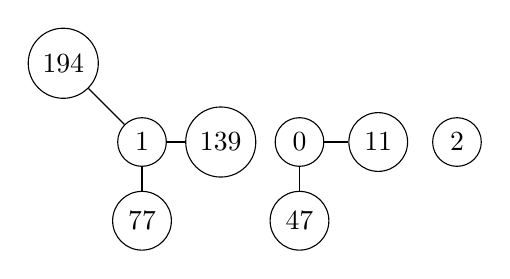
\begin{tikzpicture}

\tikzset{vertex/.style = {shape=circle,draw,minimum size=1.5em}}
\tikzset{edge/.style = {-,> = latex'}}
\node[vertex] (1) at (0,0)  {1};
\node[vertex] (194) at (-1,1)  {194};
\node[vertex] (77) at (0,-1)  {77};
\node[vertex] (139) at (1, 0) {139};
\node[vertex] (0) at (2, 0) {0};
\node[vertex] (47) at (2, -1) {47};
\node[vertex] (11) at (3, 0) {11};
\node[vertex] (2) at (4, 0) {2};
%edges
\draw[edge] (1) to (77);
\draw[edge] (1) to (139);
\draw[edge] (1) to (194);
\draw[edge] (0) to (47);
\draw[edge] (0) to (11);
\end{tikzpicture}
\end{center}

\begin{enumerate}[label=\alph*]
\item (10\%) Completa su representación utilizando listas de adyacencia:
\\
\textbf{Pista: La pregunta NO es calcular la clausura transitiva del grafo, sino la
lista de las adyacencias, es decir, la lista de los vecinos.}
\\
$0 \rightarrow 11 \rightarrow 47$
\\
$1 \rightarrow$
\\
$2 \rightarrow$
\\
$11 \rightarrow$
\\
$47 \rightarrow$
\\
$77 \rightarrow$
\\
$139 \rightarrow$
\\
$194 \rightarrow$
\end{enumerate}
\end{multicols}

\end{document}